\section{Introduction}

\subsection{Description de la societ\'e}
Australian Semiconductor Technology Company (ASTC) est un fournisseur mondial des solutions logicielles et matériels pour les systèmes embarqués. Cette société propose des services de conception, validation et vérification des systèmes sur puces et les circuits intégrés. Elle a développé son outil VLAB, qui fournit des solutions innovantes, pour la simulation des logiciels embarqués sur les plateformes Hardware virtuelles. La société a son siège à Adélaïde en Australie, elle possède des bureaux et des centres de R\&D à Toulouse, Tokyo, Illinois, Austin, et Texas.  

ASTC Desing partners a été créée à Toulouse par Nicolas Broueilh et Éric Faure en 2014. Cette partie est plus focalis\'ee en la conception de logiciel embarqué, surtout la virtualisation de hardware avec VLAB Works. Le produit le plus développé est la toolbox\footnote{Un toolbox de VLAB est une compilation des librairies qui ajoutent des modèles de simulation pour VLAB, par exemple, le toolbox Ethernet nous donne des nœuds Ethernet, ports et la classe de trame Ethernet pour l'envoie d'information.} \textit{AURIX} qui est capable de virtualiser la famille \textit{aurix} de \textit{Infineon Technologies AG}. Dans la figure \ref{fig:vlab-presentation} on peut voir un exemple de vlab. 

VLAB utilise python2 pour accéder à tous les éléments de hardware virtuel et évènements de la simulation comme les ports du microcontrôleur, registres, connections virtuelles, temps de simulation, points d'arrête, entre autres. Pour les modèles de simulation il est utilisé $C++$ avec la librairie SystemC\cite{sysc}. Il y existe une API de SystemC pour python2 en raison de développer des modèles plus rapidement mais moins performantes que celles en SystemC. 
\begin{figure}[!htb]
    \centering
        \subfigure[Logo de Vlab.]{
\includegraphics [width=2.5in]{img/VLAB_Works.png}}
        \subfigure[Vlab en marche.]{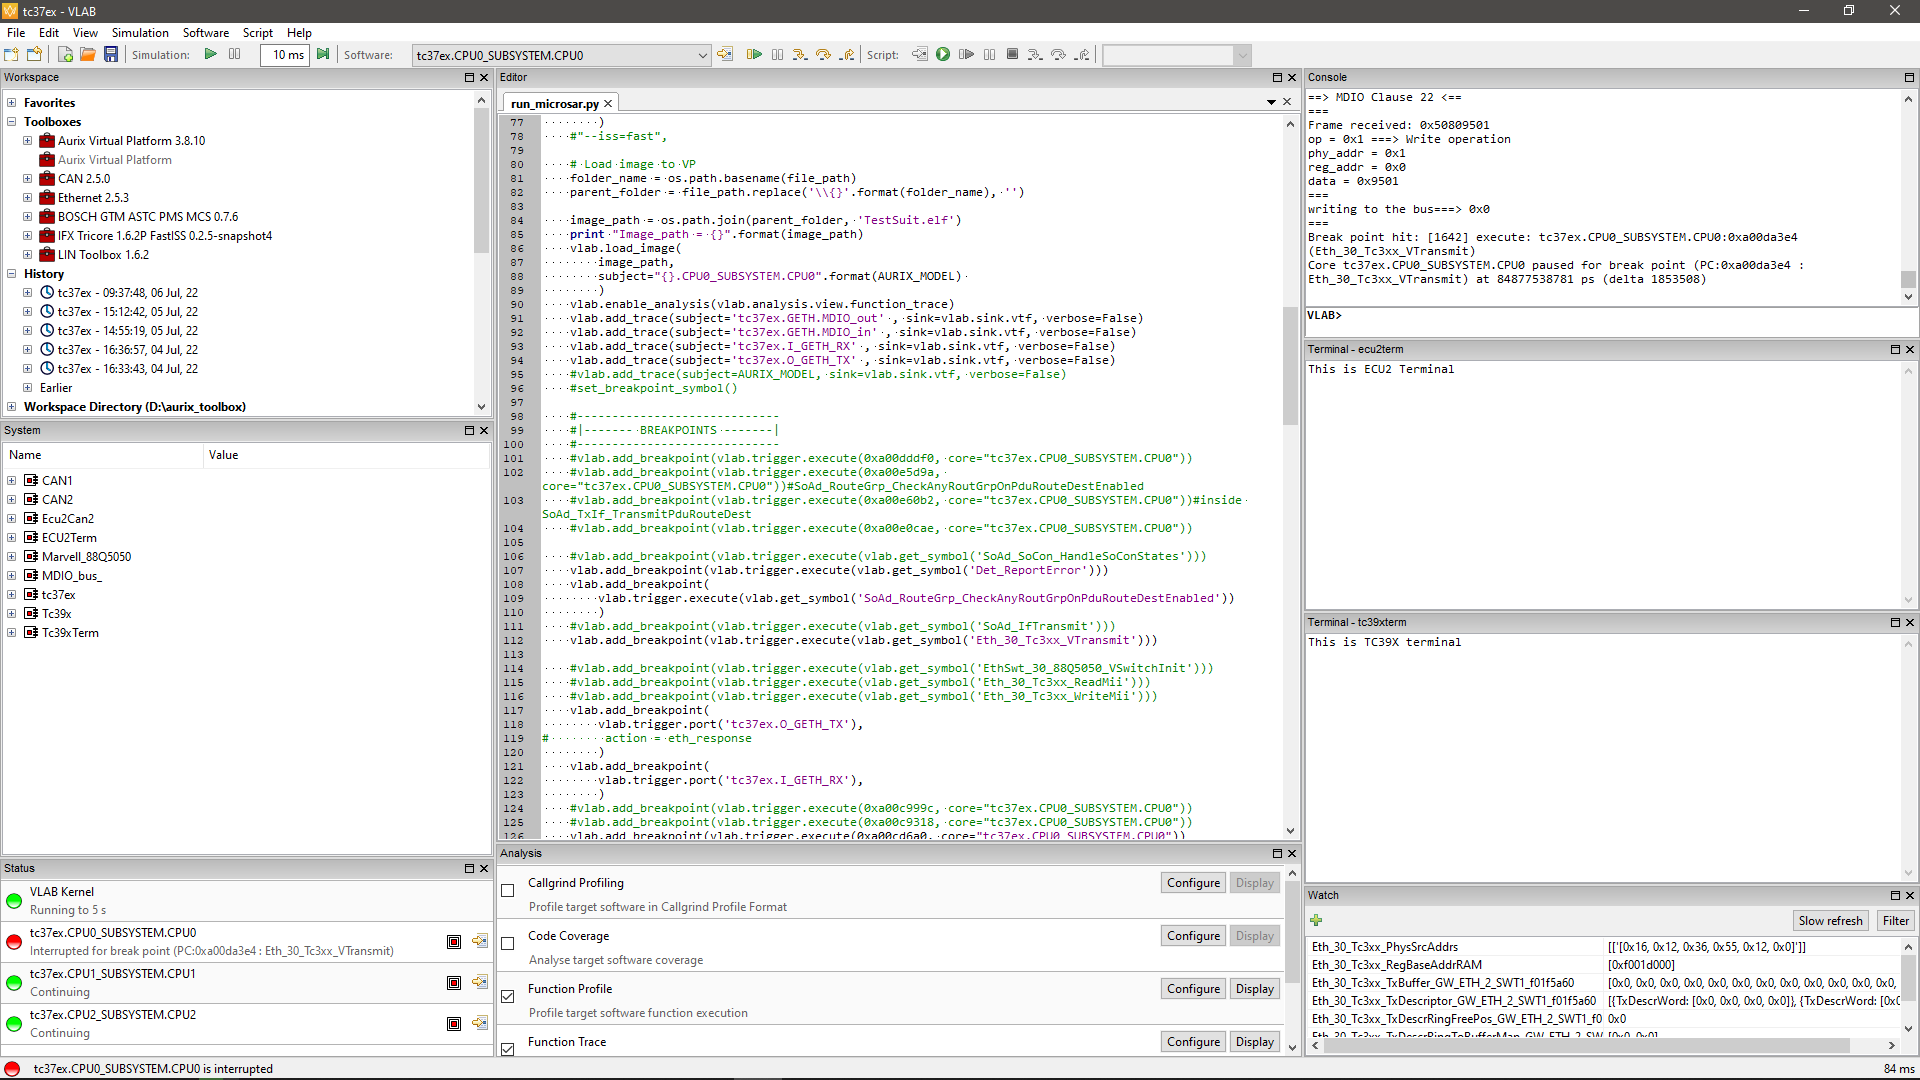
\includegraphics [width=5in]{img/vlab.png}}
    \caption{Vlab works}
    \label{fig:vlab-presentation}
\end{figure}
